\section{Integrale di Lebesgue}
\chapquote{``I have to pay a certain sum, which I have collected in my pocket. I take the bills and coins out of my pocket and give them to the creditor in the order I find them until I have reached the total sum. This is the Riemann integral. But I can proceed differently. After I have taken all the money out of my pocket I order the bills and coins according to identical values and then I pay the several heaps one after the other to the creditor. This is my integral."}{Henri Lebesgue}

\subsection{Simple Functions}
\subsubsection{(def) Simple and measurable function}
Considerando uno spazio misurabile $(X,\mathcal M)$,\\
$$s:X\to \overline{\mathbb R}$$
è semplice (e misurabile) se:
\begin{itemize}
    \item $s$ è una funzione misurabile
    \item $s(X)=\{a_1,a_2,a_3,\dots,a_k\}$ è un set finito di elementi, dove $a_i\in \overline{\mathbb R}\quad \forall i = 1,\dots, k$ con $a_i\neq a_j$ per ogni $i\neq j$.
\end{itemize}
\textbf{Forma canonica}
$$s(x)=\sum_{i=1}^k a_i\cdot \rchi_{D_i}(x)$$
dove:
\begin{itemize}
    \item $D_i=\{x\in X: s(x)=a_i\}$
    \item $D_i\cap D_j=\emptyset\quad \forall i\neq j$
    \item $X=\bigcup_{i=1}^k D_i$
\end{itemize}
\begin{center}
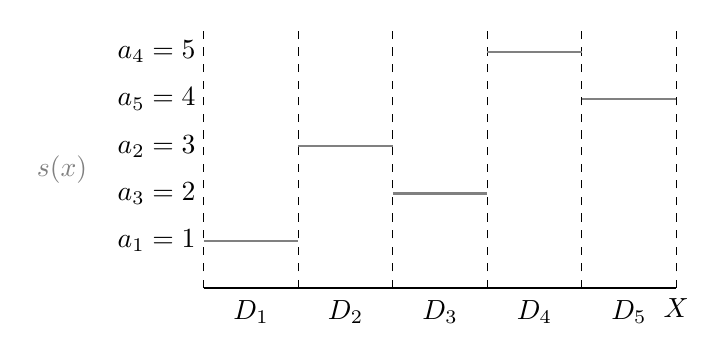
\begin{tikzpicture}[scale=0.6]
    % Define the a_i values
    \def\aone{1}
    \def\atwo{3}
    \def\athree{2}
    \def\afour{5}
    \def\afive{4}
    
    % Define the coordinates for X and D_i sets
    \draw[thick] (0,0) -- (10,0) node[below] {$X$}; % X axis
    \foreach \x in {0, 2, 4, 6, 8, 10} % Vertical lines for D_i sets
        \draw[dashed] (\x,0) -- (\x,5.5);
    
    % Label the D_i sets
    \node at (1,-0.5) {$D_1$};
    \node at (3,-0.5) {$D_2$};
    \node at (5,-0.5) {$D_3$};
    \node at (7,-0.5) {$D_4$};
    \node at (9,-0.5) {$D_5$};
    
    % Plot the values of s(x)
    \draw[thick,gray] (0,\aone) -- (2,\aone); % a_1
    \draw[thick,gray] (2,\atwo) -- (4,\atwo); % a_2
    \draw[thick,gray] (4,\athree) -- (6,\athree); % a_3
    \draw[thick,gray] (6,\afour) -- (8,\afour); % a_4
    \draw[thick,gray] (8,\afive) -- (10,\afive); % a_5
    
    % Label the a_i values
    \node at (-1,\aone) {$a_1=1$};
    \node at (-1,\atwo) {$a_2=3$};
    \node at (-1,\athree) {$a_3=2$};
    \node at (-1,\afour) {$a_4=5$};
    \node at (-1,\afive) {$a_5=4$};

    % y-axis label
    \node[thick, gray] at (-3,2.5) {$s(x)$};

    
\end{tikzpicture}
\end{center}
\subsubsection{(thm) Simple Approximation Theorem (SAT) (*)}
Presi
\begin{itemize}
    \item $(X,\mathcal M)$ spazio misurabile
    \item $f:X\to [0,+\infty]$ funzione misurabile
\end{itemize}
Allora esiste una successione di funzioni semplici misurabili che approssimano dal basso la funzione $f$.
\\ Ovvero:\\
$\exists \{s_n\}_{n\in \mathbb N}$ t.c. $s_i$ è funzione semplice e misurabile $\forall i\in \mathbb N$ e:
$$0\le s_1\le s_2\le \dots \le s_n\le \dots \le f$$ pointwise (ovvero $\forall x \in X$).\\
Si ha quindi che 
$$\lim_{n\to +\infty} s_n(x)=f(x) \quad \forall x\in X$$
Inoltre, se $f$ è bounded, la convergenza è uniforme:
$$\sup_{x\in X}\vert s_n(x)-f(x)\vert \xrightarrow[n\to +\infty]{} 0$$
\subsubsection{(def) Integrale di Lebesgue}
Consideriamo uno spazio di misura $(X,\mathcal M, \mu)$.\\
Sia $s:X\to [0,+\infty]$ una funzione semplice e misurabile:
$$s(x)=\sum_{i=1}^k a_i\cdot \rchi_{D_i}(x)$$
Con $a_i\ge 0$ e $D_i\in \mathcal M$.\\
Sia $E\in \mathcal M$.\\
L'integrale di Lebesgue di $s$ su $E$ è:
$$\int_{E}s\ \mathrm{d\mu}\coloneqq\sum_{i=1}^k a_i\cdot\mu(D_i\cap E)$$

\subsubsection{(prop) Basic properties of the Lebesgue's integral}
Siano $N,E,F\in \mathcal M$, $s_1,s_2:X\to [0,+\infty]$ delle funzioni semplici e misurabili.\\
Allora:\\
\begin{enumerate}
    \item Nullità su insiemi di misura nulla.\\$$\mu(N)=0\implies \int_Ns_1\mathrm{d}\mu=0$$
    \item Omogeneità rispetto alla moltiplicazione per una costante positiva. \\ Data $0\le c\le +\infty $, $$\int_E c\cdot s_1\mathrm{d}\mu=c\int_E s_1\mathrm{d}\mu$$
    \item Additività rispetto alla somma.
    $$\int_E(s_1+s_2)\mathrm{d}\mu=\int_Es_1\mathrm{d}\mu+\int_Es_2\mathrm{d}\mu$$
    \item Monotonicità$$s_1\le s_2\implies \int_Es_1\mathrm{d}\mu\le\int_Es_2\mathrm{d}\mu$$
    \item Monotonia sugli insiemi$$E\subset F\implies \int_Es_1\mathrm{d}\mu\le\int_Fs_1\mathrm d\mu$$ 
\end{enumerate}
\subsubsection{(prop) The integral of non negative simple measurable functions is a measure (*)}
Data $s:X\to[0,+\infty]$, semplice e misurabile,\\
Definendo $\varphi:\mathcal M\to[0,+\infty]$ tale che:
$$\varphi(E)=\int_E s\ \mathrm{d}\mu\quad\text{con } E\in \mathcal M$$
Allora $\varphi$ è una misura su $(X,\mathcal M)$.
\subsubsection{(def) Integrale di funzioni misurabili non negative}
Data una funzione misurabile $f:X\to[0,+\infty]$, $E\in\mathcal M$
$$\int_E f\ \mathrm{d}\mu\coloneqq \sup\Big\{\int_E s\ \mathrm d\mu: s \text{ semplice e misurabile, } 0\le s\le f\Big\}$$
\subsubsection{(prop) Disuguaglianza di Chebyshev (*)}
Considerando: 
\begin{itemize}
    \item uno spazio di misura completo $(X,\mathcal M,\mu)$
    \item $f:X\to[0,+\infty]$, misurabile
    \item $0<c<+\infty$ 
\end{itemize}
Allora
$$\mu\Big(\{x\in X:f(x)\ge c\}\Big)\le\frac1c\int_{\{f\ge c\}}f\ \mathrm{d}\mu \le \frac1c\int_X f\ \mathrm{d}\mu$$
\subsubsection{(lemma) Vanishing lemma (*)}
Dati:
\begin{itemize}
    \item $f:X\to[0,+\infty]$ una funzione misurabile
    \item $E\in\mathcal M$
\end{itemize}
Allora vale:
$$\int_Ef\ \mathrm{d}\mu=0\iff f(x)=0$$ per a.e. $x\in E$
\subsubsection{(lemma) Condizione di finitezza per l'integrale rispetto a una misura (*)}
Data una funzione $f:X\to [0,+\infty]$ misurabile, allora:
$$\int_X f\ \mathrm d\mu<+\infty \iff \mu\Big(\Big\{x\in X:f(x)=+\infty\Big\}\Big)=0$$
\subsection{Convergence Theorems}
\subsubsection{(thm) Monotone Convergence Theorem (Beppo Levi's)}
Given a function $f_n:X\to [0,+\infty]$ measurable $\forall n\in \mathbb N$,\\
Assume:
\begin{enumerate}[label=\roman*.]
    \item $f_n(x)\le f_{n+1}(x)$ for a.e. $x\in X$
    \item $f_n(x)\xrightarrow[n\to+\infty]{} f(x)$ for $\mu$-almost every $x\in X$
\end{enumerate}
Then:
$$\int_X f\ \mathrm d\mu=\lim_{n\to +\infty}\int_X f_n\ \mathrm d\mu$$
Il significato è che presa una successione di funzioni non negative crescente e convergente a una funzione $f$ quasi ovunque, allora l'integrale del limite è pari al limite dell'integrale della successione per $n \to +\infty$

\subsubsection{(corollary) Monotone convergence for series (*)}
Data una funzione $f_n:X\to [0,+\infty]$ misurabile $\forall n\in \mathbb N$
$$\int_X\Big(\sum_{n\in \mathbb N}f_n\Big)\mathrm d\mu=\sum_{n\in\mathbb N}\Big(\int_X f_n \ \mathrm d\mu\Big )$$
\subsubsection{(prop) The integral of a non negative measurable function is a measure (*)}
Presa $\Phi : X\to [0,+\infty]$ misurabile, $E\in \mathcal M$,\\
Si definisce:
$$\nu(E)=\int_E \Phi\ \mathrm d\mu$$
Allora $\nu$ è una misura su $(X,\mathcal M)$,\\
Inoltre (data $f:X\to[0,+\infty]$ misurabile),
$$\int_X f\ \mathrm d\nu = \int_X f\Phi \ \mathrm d\mu$$
\subsubsection{(lemma) Fatou's Lemma (*)}
Considerando:
\begin{itemize}
    \item uno spazio di misura $(X,\mathcal M,\mu)$ completo
    \item $f_n:X\to [0,+\infty]$ misurabile $\forall n\in \mathbb N$
\end{itemize}
Allora:
$$\int_X\Big ( \liminf_n f_n\Big ) \mathrm d\mu\le \liminf_n\Big(\int_X f_n\ \mathrm d\mu\Big)$$
\subsubsection{(def) Funzione integrabile e insieme di funzioni integrabili L1}
$f:X\to \overline{\mathbb R}$ è integrabile su $X$ se:
\begin{itemize}
    \item è misurabile
    \item l'integrale di Lebesgue del modulo della funzione è finito e positivo$$\int_X\vert f\vert \mathrm d\mu <+\infty$$
\end{itemize}
Definiamo quindi
$$\mathcal L^1(X,\mathcal M,\mu)\coloneqq\{f:X\to \overline{\mathbb R}\ |\  f \text{ Lebesgue integrabile}\}$$ 
ovvero l'insieme delle funzioni integrabili secondo Lebesgue.
\subsubsection{(def) integrale di Lebesgue con decomposizione in parti positive e negative}
Per $f\in \mathcal L^1(X,\mathcal M,\mu)$ e $E\in \mathcal M$, definiamo:
$$\int_X f\ \mathrm{d}\mu\coloneqq \int_X f^+\mathrm d\mu-\int_X f^-\mathrm d\mu$$
$$\int_E f\mathrm d\mu \coloneqq \int_X f\rchi_E \mathrm d\mu$$
\subsubsection{(prop) implicazioni della misurabilità (*)}
\begin{enumerate}[label=\roman*]
    \item $f\in \mathcal L^1 \iff |f|\in \mathcal L^1 \iff f^+,f^-\in \mathcal L^1$
    \item triangular inequality $$0\leq \Big\vert\int_X f \mathrm d\mu\Big|\leq \int_X|f|\mathrm d\mu$$
\end{enumerate}
\subsubsection{(prop) $\mathcal L^1$ is a vector space}
\begin{enumerate}
    \item $\mathcal L^1(X,\mathcal M,\mu)$ è uno spazio vettoriale reale
    \item $\int_X \mathrm d\mu:\mathcal L^1(X,\mathcal M,\mu)\to \mathbb R$ è lineare
\end{enumerate}
\subsubsection{(thm) Full optional Vanishing lemma (*)}
Si consideri $(X,\mathcal M,\mu)$ completo, $f,g\in \mathcal L^1(X,\mathcal M,\mu)$.
Allora, $$f=g \text{ a.e. }\iff \int_X |f-g|\mathrm d\mu =0\iff \int_E(f-g)\mathrm d\mu=0\quad \forall E\in \mathcal M$$
\subsubsection{(thm) Lebesgue's Dominated Convergence Theorem}
Sia $(X,\mathcal M,\mu)$ completo.
$\{ f_n\}_{n\in \mathbb N}, \ f_n:X\to \overline{\mathbb R}$ misurabile.

Assumendo:
\begin{itemize}
    \item $f_n(x)\to f(x)$ a.e. $x\in X$
    \item $\exists g\in \mathcal L^1(x)$ tale che $|f_n(x)|\leq g(x)$ a.e. $x\in X$
\end{itemize}
Allora,
$$f\in \mathcal L^1(x) \text{ e }\lim_{n\to +\infty}\int_X|f_n-f|\mathrm d\mu=0$$
$$\lim_{n\to +\infty}\int_Xf_n\mathrm d\mu=\int_X f\mathrm d\mu$$

\subsubsection{(rmk) Dominanted convergence for a.e. bounded functions}
Se $\mu(x)<+\infty \implies$ constants are integrable. Then, if $f_n(x)|\leq M\ a.e.$,
$$\lim_n\int_X f_n=\int_X\lim_n f_n$$
Allora conviene usare semplicemente $g(x) = M$.
\subsubsection{(corollary) Dominated convergence for series}
$\{f_n\}_n\subset \mathcal L^1(X,\mathcal M,\mu)$

Se $\sum_n\int_X |f_n|\mathrm d\mu <+\infty \implies$ $$ \int_X\Big ( \sum_n f_n\Big ) \mathrm d\mu = \sum_n\Big ( \int_X f_n \mathrm d\mu\Big )$$
\subsection{Riemann's vs Lebesgue's integrals}
\subsubsection{(thm) Riemann's proper integrability implies Lebesgue's integrability}
Siano:
\begin{itemize}
    \item $I=[a,b]\subset \mathbb R$
    \item $f:I\to \mathbb R$ Riemann-integrable
\end{itemize}
Allora,
$$f\in \mathcal L^1(I,\mathcal L(I),\lambda)$$
e
$$\int_{[a,b]} f \mathrm d\lambda = \int_a^b f(x) \mathrm dx$$
\subsubsection{(thm) Riemann's $\int_\alpha^\beta|f|\mathrm dx$ (generalized) convergence implications}
Siano $I=(\alpha, \beta)$, $-\infty\leq \alpha <\beta \leq +\infty$\\
Se $|f|$ è Riemann-integrabile in senso generalizzato, allora
\begin{enumerate}
    \item $f \in \mathcal L^1$
    \item $\int_{(\alpha, \beta)} f\mathrm d\lambda = \int_\alpha^\beta f(x)\mathrm dx$
\end{enumerate}
\subsubsection{(rmk) What if $\int_\alpha^\beta|f|\mathrm dx$ (generalized) diverges?}
Se l'integrale di Riemann generalizzato di $|f|$ diverge $\implies \int_{(\alpha,\beta)}|f|\mathrm d\lambda =+\infty$\\
Ma $\int_{(\alpha,\beta)} f\mathrm d\lambda$ non è definito (a meno che $f = \pm |f|$) e $\int_{(\alpha,\beta)} f\mathrm d\lambda $ non è correlato con $\int_\alpha^\beta f(x)\mathrm dx$.\\
\textbf{Example} $f:(0,+\infty)\to \mathbb R$, $f(x)=\frac{\sin x}x$
